\section{Apéndice} \label{cap:apendice}
\subsection{A: Enunciado}
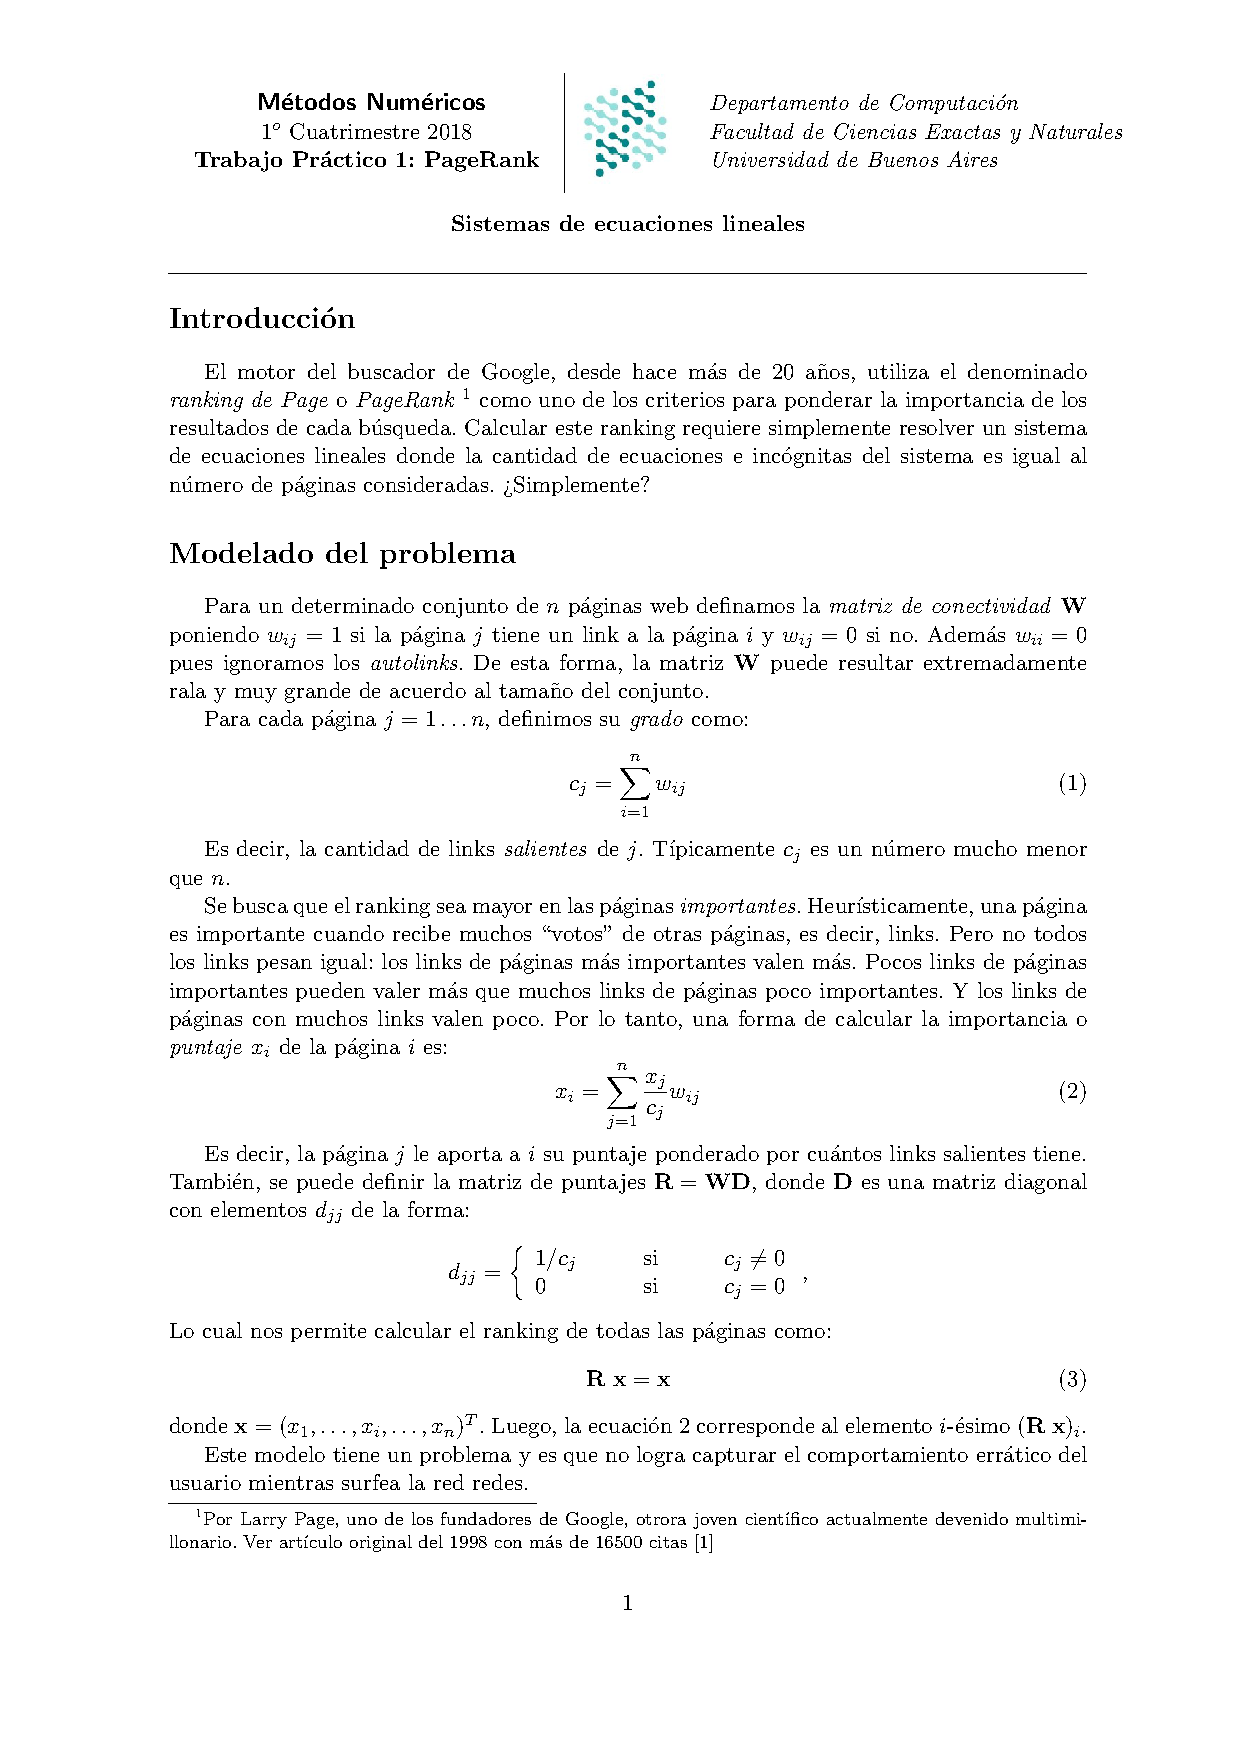
\includepdf[pages=-]{../enunciado/Enunciado_TP1.pdf}

\subsection{B: Código}

\begin{center}
{\small Matriz.h\\}
\end{center}
\begin{lstlisting}

const double epsilon = 0.000000001;

/// Indexa de 1 a n/m ///

class Matriz
{

public:

    Matriz();

    Matriz(int, int);

    ~Matriz();

    int Filas();

    int Columnas();

    Matriz & Set(double val, int fila, int col); 

    double Get(int, int) const;

    void escalar(double k);    

    vector<double> multiply(const vector<double> & x) const;

    void resolver(vector<double> & ranking, vector<double> &b);

    void eliminacionGaussiana(vector<double>& b);

    void backwardSubstitution(vector<double>& ranking, vector<double>& b);

    friend bool operator == (const Matriz & a, const Matriz & b);

    friend bool operator != (const Matriz & a, const Matriz & b);

    friend vector<double> operator * (const Matriz & a, const vector<double> & b);

    friend ostream & operator << (ostream & os, const Matriz & matrix);

    void columnaPorMenosPSobreSuGrado(vector<int>& grados, double p);

    int GetNoNulos();


private:
    
    vector<list<pair<int,double> > >  filas_ptr;
    int nnz;

    int filas;
    int columnas;

    void construct(int fila, int columna);
    void validarCoordenadas(int fila, int col) const;


};


\end{lstlisting}

\newpage

\begin{center}
{\small Matriz.cpp\\}
\end{center}
\begin{lstlisting}


#include "Matriz.h"


Matriz::Matriz()
{
    filas = 0;
    columnas = 0;
}

Matriz::Matriz(int filas, int columnas)
{
    this->construct(filas, columnas);
}

Matriz::~Matriz()
{
   
}

int Matriz::Filas()
{
    return filas;
}

int Matriz::Columnas()
{
    return columnas;
}

void Matriz::construct(int filas, int columnas)
{
    if (filas < 1 || columnas < 1) {
        throw "La dimension de la matriz no puede ser cero o negativa";
    }

    this->filas = filas;
    this->columnas = columnas;

    list<pair<int,double> > lista;
    vector<list<pair<int,double> > > vec(filas,lista);

    filas_ptr = vec;

    nnz = 0;
}


Matriz & Matriz::Set(double val, int fila, int col)
{   
 
        this->validarCoordenadas(fila, col);

        if (abs(val) < epsilon){
           auto it = filas_ptr[fila-1].begin();
           for (it; it != filas_ptr[fila-1].end() && it->first != col; ++it){}
           if (it != filas_ptr[fila-1].end()){
                
                filas_ptr[fila-1].erase(it);
                --nnz;
                }
        }else{
            auto it = filas_ptr[fila-1].begin();


            for (it; it != filas_ptr[fila-1].end()&& it->first < col; ++it){}
            if (it != filas_ptr[filas-1].end() && it->first == col)
            {
                it->second = val;

            }else{
                pair<int,double> nodo;
                nodo.first = col; nodo.second = val;
                if (it == filas_ptr[filas-1].end())
                {   
                       filas_ptr[filas-1].emplace(it,nodo);
                }else{
                    if (it->first == col)
                    {
                         it->second = val;
                    }else{
                        filas_ptr[filas-1].insert(it,nodo);
                    }

                }

                 ++nnz;
            }
      
        }

    return *this;
}



double Matriz::Get(int fila, int col) const
{
    this->validarCoordenadas(fila, col);

    auto it = filas_ptr[fila-1].begin();
    for (it; it != filas_ptr[fila-1].end()&& it->first != col; ++it ){}

    if ( it != filas_ptr[fila-1].end())
    {

            return (it->second);
    }

    return 0;
}

int Matriz::GetNoNulos(){

    return nnz;
}

void Matriz::escalar(double k)
{
    for (int i = 0; i < filas; ++i)
    {
        for (auto it = filas_ptr[i].begin(); it != filas_ptr[i].end(); ++it)
        {
            it->second = it->second*k;
        }
    }
}

vector<double> Matriz::multiply(const vector<double> & x) const
{
    vector<double> res (filas, 0.0);

    for (int i = 0; i < filas; ++i)
    {
        double acum = 0.0;
        for (auto it = filas_ptr[i].begin(); it != filas_ptr[i].end(); ++it)
        {
            acum = acum + it->second*x[it->first];
        }
        res[i] = acum;
    }

    return res;
}


void Matriz::validarCoordenadas(int fila, int col) const
{
    if (fila < 1 || col < 1 || fila > this->filas || col > this->columnas) {
        throw "Coordenadas fuera del rango";
    }
}


bool operator == (const Matriz & a, const Matriz & b)
{
    return a.filas_ptr == b.filas_ptr;
}


bool operator != (const Matriz & a, const Matriz & b)
{
    return !(a == b);
}


ostream & operator << (ostream & os, const Matriz & matrix)
{
    for (int i = 1; i <= matrix.filas; i++) {
        for (int j = 1; j <= matrix.columnas; j++) {
            if (j != 1) {
                os << " ";
            }

            os << matrix.Get(i, j);
        }

        if (i < matrix.filas) {
            os << endl;
        }
    }

    return os;
}

vector<double> operator * (const Matriz & a, const vector<double> & b) {

    return a.multiply(b);
}


void Matriz::columnaPorMenosPSobreSuGrado(vector<int>& grados, double p){

   for (int i = 0; i < filas; ++i)
    {   
        for(auto it = filas_ptr[i].begin(); it != filas_ptr[i].end(); ++it){
            it->second = (-1.0)*(it->second)*p/grados[it->first-1];
        }

    }
}

void Matriz::resolver(vector<double> & ranking, vector<double> &b){

    this->eliminacionGaussiana(b);

    this->backwardSubstitution(ranking,b);

}


void Matriz::eliminacionGaussiana(vector<double>& b){

    for (int k = 0; k < filas; ++k)
    {       

        for (int i = k+1; i < filas; ++i)
          {
              //iterador de la fila k. La que es usada para restarle. Es el primero de la fila porque hasta la columna k-1 fue triangulada.
              auto it_k = filas_ptr[k].begin();
              // iterador de la fila de las columnas debajo del pivot. Si el primer valor es de la columna k+1 entonces tengo que anularlo.
              auto it_i = filas_ptr[i].begin();


             if (it_i->first == k+1)
              {

                  double coef = (double) it_i->second/it_k->second; 

                    for (; it_k != filas_ptr[k].end(); ++it_k)
                    {
                         //si en la fila i a la que le quiero anular la col k+1 hay elementos entre las columnas de la fila k los dejo como estan.
                        
                         while(it_i != filas_ptr[i].end() && (it_i->first < it_k->first)){
                            ++it_i;
                         }

                         double resta = 0.0;

                         //si estamos en la msima columna resto.
                         if (it_i != filas_ptr[i].end() &&  (it_i->first == it_k->first))
                         {
                            resta = it_i->second - coef*it_k->second;
                            if(abs(resta) > epsilon){ //actualizo valor si es distinto de cero e incrmento iterador.
                                it_i->second = resta;
                                 ++it_i;
                            }
                            else{ //si es cero lo scao.
                                auto it_temp = it_i;
                                ++it_i;
                                filas_ptr[i].erase(it_temp);
                                --nnz;
                            }
                           
                         }else{ // columna de i es mayor a columna de k. No hay elem no nulo  y tengo que insertarlo.

                            double resta = (double) (-1.0)*coef*it_k->second;

                            if(abs(resta) > epsilon) {
                               
                                pair<int,double> nodo; nodo.first = it_k->first; nodo.second = resta;
                                filas_ptr[i].insert(it_i, nodo);
                                ++nnz;
                            }  

                         }
      
                    }
                    b[i] = b[i] - coef*b[k];

              }
            }  
    }

}

void Matriz::backwardSubstitution(vector<double>& ranking, vector<double>& b){

    double acum = 0.0;

    for (int k = filas-1; k >= 0; --k)
    {
        // indice en vals donde empieza la fila k y por lo tanto a_k_k.       

        //recorro la fila en busca de coeficientes no nulos que multipliquen a las
        // x_l mayores que a x_i_i.

        auto it = filas_ptr[k].begin();
        double a_k_k = it->second;
        for (it = ++it; it != filas_ptr[k].end(); ++it){
            acum = acum + it->second*ranking[it->first -1];

        }

        //resto b_i menos el acum y lo divido por el coef de a_i_i.

        ranking[k] = (double) ((b[k]-acum) / a_k_k);
        acum = 0.0;

    }

 }
 
\end{lstlisting}

\newpage

\begin{center}
{\small PageRank.h\\}
\end{center}
\begin{lstlisting} 

class PageRank
{

public:

    PageRank();

    PageRank(Matriz& W, vector<int> & grado_de_paginas);

    ~PageRank();

    Matriz& GetMatrizDeConectividad();

    vector<double>& GetRanking();

    vector<int >& GetGradoDePaginas();

    int getCantDePaginas();

    int obtenerGradoPagina(int);

    void calcularRanking(double p);	

private:
    Matriz matrizDeConectividad;
    vector<double > ranking;   
    vector<int > gradoDePaginas;    
    int cantDePaginas; 

};

\end{lstlisting}



\begin{center}
{\small PageRank.cpp\\}
\end{center}
\begin{lstlisting} 

PageRank::PageRank()
{
    matrizDeConectividad = Matriz();
    gradoDePaginas = vector<int>();
    ranking = vector<double>();
    cantDePaginas = 0;
}

PageRank::PageRank(Matriz& W, vector<int> & grado_de_paginas){

    matrizDeConectividad = W;
    gradoDePaginas = grado_de_paginas;
    cantDePaginas = W.Filas();
    ranking = vector<double>(cantDePaginas);

}

PageRank::~PageRank()
{
}

bool contienePagina(vector<pair<int, int> > paginas, int pagOrigen)
{
    bool res = false;
    for(int i = 0; i < paginas.size(); i++) if(paginas[i].first == pagOrigen) res=true;
    return res;
}

int obtenerIndicePagina(vector<pair<int, int> > paginas, int pagOrigen)
{
    int res;
    for(int i = 0; i < paginas.size(); i++) if(paginas[i].first == pagOrigen) res=i;
    return res;
}

int PageRank::obtenerGradoPagina(int pagOrigen)
{
    int res;
    res = gradoDePaginas[pagOrigen-1];
    return res;
}


Matriz& PageRank::GetMatrizDeConectividad()
{
    return matrizDeConectividad;
}

vector<double >& PageRank::GetRanking()
{
    return ranking;
}

vector<int >& PageRank::GetGradoDePaginas()
{
    return gradoDePaginas;
}

int PageRank::getCantDePaginas()
{
    return cantDePaginas;
}

double norma(vector<double> &v)
{
    double res = 0;
    for(long i = 0; i < v.size(); i++) res += v[i]*v[i];
    return (double) sqrt(res);
}

void divEscalar(vector<double> &v, double alpha)    
{
    if(alpha!=0)
        for(int i = 0; i < v.size(); i++) v[i] = (double) (v[i]/alpha);
}

double normaManhattan(vector<double> &v)
{
   double res = 0;
    for(int i = 0; i < v.size(); i++)res += abs((double)v[i]);
    return res;
}

void normalizar(vector<double> &V){

    double nrm = (double) normaManhattan(V);
    divEscalar(V, nrm);
}

void PageRank::calcularRanking(double p)
{

    vector<double> b(this->cantDePaginas,1);

    // matrizDeCOnectividad = -pAD
    this->matrizDeConectividad.columnaPorMenosPSobreSuGrado(this->gradoDePaginas,p);

    //matrizDeConectividad = matrizDeConectividad + i. La que queremos resolver.
    for (int i = 1; i <= this->cantDePaginas; ++i)
        {
            this->matrizDeConectividad.Set(1,i,i);
        }    

    vector<double> solucion(cantDePaginas);

    this->matrizDeConectividad.resolver(this->ranking,b);

    normalizar(ranking);

}

\end{lstlisting}

\newpage